\section{Principes radar}
% La proposition de ce plan peut-être adaptée selon les avis, notamment sur la partie hardware
\subsection{Généralités}
% S'inspirer de l'existant, ajuster (ajouter le SNR brièvement)

Avant d’aborder les techniques avancées d’imagerie SAR, il est utile de rappeler les notions clés des systèmes radar. Un radar émet une onde électromagnétique directive à l’aide d’une antenne, représentée par les rectangles noirs dans la figure \ref{fig:schema_base_radar}. Lorsqu’elle rencontre une cible, une partie de l’énergie est renvoyée sous forme d’échos — indiqués en rouge — qui se propagent avec des amplitudes et des phases variables. Ces échos peuvent également se réfléchir sur d’autres objets, générant des contributions secondaires. Une fraction de ces retours est recueillie par l’antenne et analysée pour extraire des informations essentielles telles que : la distance de la cible, sa vitesse relative et certains aspects de sa structure \cite{skolnik2001}.

%\begin{figure}[htbp]
%    \centering
%    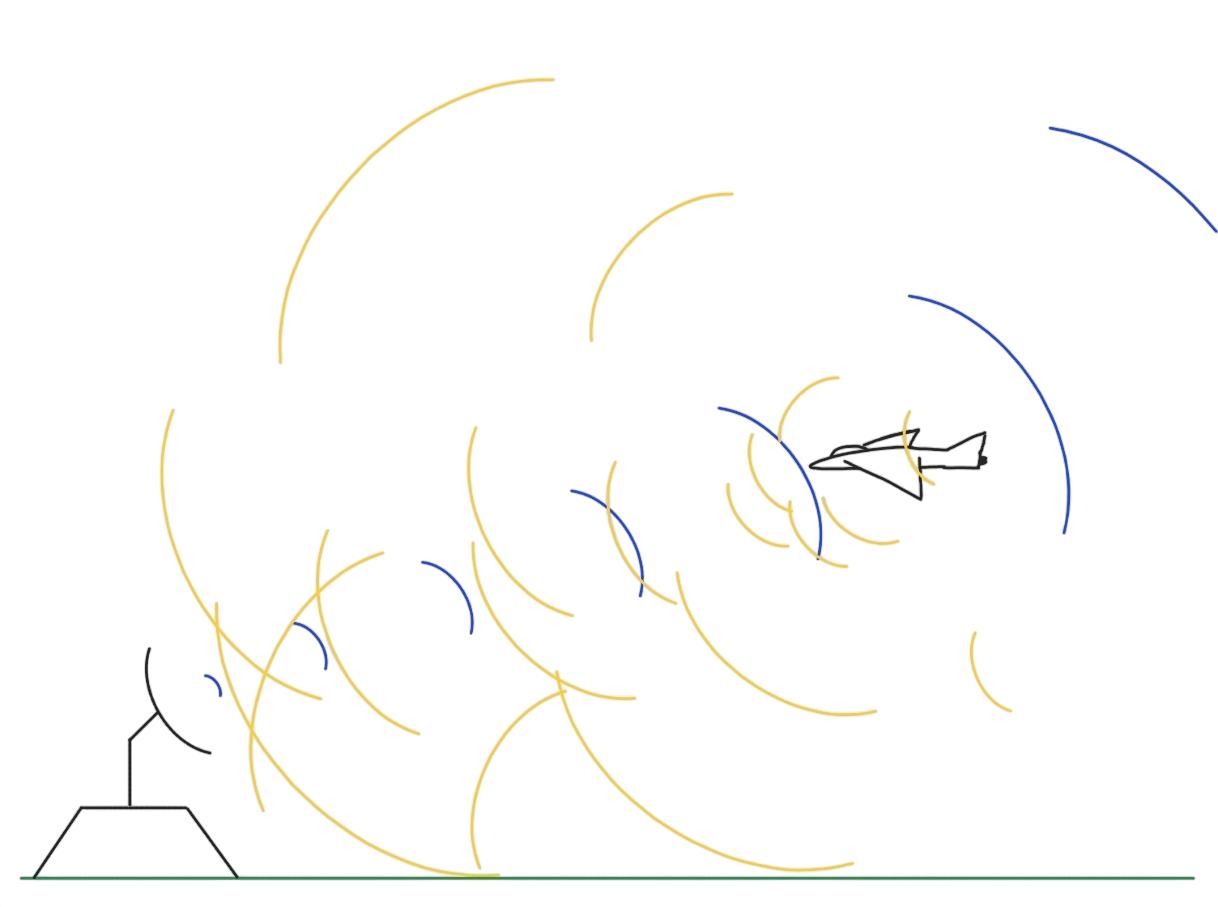
\includegraphics[width=0.5\linewidth]{src/rapport_complet/img/schema_base_radar.png}
%    \caption{Schéma d'explication des bases d'un système radar}
%    \label{fig:schema_explicatif_radar}
%\end{figure}

\begin{figure}[htbp] 
    \centering 
    \begin{tikzpicture}
    % Définir les styles
    \tikzset{
        % Faisceau émis : ÉPAISSI ET ESPACÉ
        radar beam/.style={black, line width=7.5pt, opacity=0.75, dash pattern=on 10pt off 30pt},
        % Écho principal : PLUS VISIBLE ET ESPACÉ
        echo beam/.style={red, line width=10pt, opacity=0.75, dash pattern=on 10pt off 30pt},
        % Échos diffractés : PLUS VISIBLES ET ESPACÉS
        diffracted echo/.style={red, line width=5pt, opacity=0.75, dash pattern=on 10pt off 30pt},
        ground/.style={draw=green!50!black, thick},
        axis/.style={gray, thin, ->},
        annotation/.style={black, font=\small},
        angle arc/.style={draw=gray, thick, ->, shorten < = 2pt, shorten > = 2pt}
    }
    % --- Variable pour l'angle de l'antenne ---
    \def\RadarAngle{25} % C'EST LA VARIABLE À AJUSTER (en degrés)
    % Sol
    \draw[ground] (0,0) -- (10,0) node[below right, annotation] {Sol};
    % Antenne (partie fixe)
    \draw[thick] (0.2, 0.5) -- (0.8, 0.5) -- (1, 0) -- (0, 0) -- cycle; % Base
    \draw[thick] (0.5, 0.5) -- (0.5, 1.5); % Support vertical     
    % \node at (0.5, 3.2) [above, annotation] {Antenne Radar};     
    % Définition du point de pivot de l'antenne
    \coordinate (radar_pivot) at (0.5, 1.5);
    % --- Partie rotative de l'antenne (Bras + Parabole) ---
    % (INCHANGÉ, comme demandé)
    \begin{scope}[shift={(radar_pivot)}, rotate=\RadarAngle]
        % Le bras qui tient le point focal (longueur 0.5cm)
        \draw[thick] (0,0) -- (0.5, 0);    
        % La parabole
        \draw[thick] (0.75, 0.65) arc (130:230:0.8cm and 0.8cm);    
        % Définir le point focal RELATIF au pivot
        \coordinate (radar_focal_point_relative) at (0.5, 0);      
    \end{scope} % Fin de la partie rotative
    % Point focal (émission/réception) en coordonnées absolues
    \coordinate (radar_focal_point) at ($(radar_pivot) + (\RadarAngle:0.5cm)$);
    % Position de l'avion (cible)
    \coordinate (avion_pos) at (8, 5);
    % Inclure l'image de l'avion
    \node (avion_node) at (avion_pos) {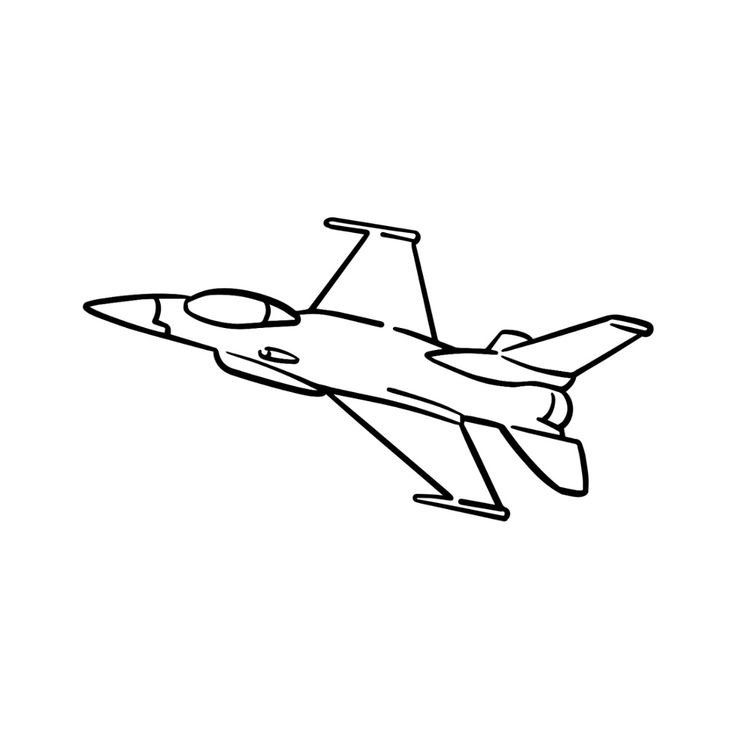
\includegraphics[width=2cm]{src/rapport_complet/img/avion.jpg}};
    % Faisceau émis (style mis à jour)
    \draw[radar beam] (radar_focal_point) -- (avion_pos);          
    % --- Échos de retour ---
    % L'écho principal qui revient à l'antenne
    \draw[echo beam] (avion_pos) -- (radar_focal_point);      
    % NOUVEAU : Échos diffractés (simples)
    \draw[diffracted echo] (avion_pos) -- ++(-5, 3);    % Vers le haut à gauche leger
    \draw[diffracted echo] (avion_pos) -- ++(-8, 0);  % horizontal à gauche
    \draw[diffracted echo] (avion_pos) -- ++(2.5, -5);  % Vers le bas à droite
    \draw[diffracted echo] (avion_pos) -- ++(-4, -4.75);    % Vers le bas à gauche
    % Annotation de la distance relative
    \draw[<->, black, thin] (radar_focal_point) -- node[above, sloped, annotation] {($R$)} (avion_pos);
    % Ligne d'élévation (Altitude)
    \draw[black, thin, densely dotted] (avion_pos) -- (avion_pos |- 0,0) node[below] {$P$};
    \draw[<->, black, thin] (avion_pos |- 0,0) -- node[right, annotation] {($h_{av}$)} (avion_pos);
    % Angle du radar (angle de site)
    \coordinate (horizontal_end) at ($(radar_focal_point) + (7.5,0)$);    
    \draw[black, dashed] (radar_focal_point) -- (horizontal_end); % Ligne horizontale à partir du foyer    
    \draw[angle arc, black] ($(radar_focal_point) + (2.5,0)$) arc (0:\RadarAngle:2.5cm) node[midway, right, annotation] {($\theta_a$)};
    % Ligne et annotation h_ant (décalées de 1 sur la droite)
    \draw[<->, black, thin] ($(radar_focal_point |- 0,0) + (1,0)$) -- node[right=1pt, annotation] {($h_{ant}$)} ($(radar_focal_point) + (1,0)$);
    \draw[<->, blue, thin] ($(avion_pos |- horizontal_end) + (-0.05,0)$) -- node[left, annotation, blue] {($h_{av_{relative}}$)} ($(avion_pos)+(-0.05,0)$);
\end{tikzpicture}
    \caption{Illustration d'un radar}
    \label{fig:schema_base_radar}
\end{figure}

\noindent La puissance reçue $P_r$ s’exprime selon l’« équation radar » classique \cite{richards2010} :

\begin{equation}
    P_r = \frac{P_t \cdot G^2 \cdot \lambda^2 \cdot \sigma_r}{(4\cdot\pi)^3\cdot R^4}.
    \label{eq:equation_radar}
\end{equation}
Où : 
\begin{description}
    \item[$P_r$] : est la puissance reçue par l'antenne [$W$]
    \item[$P_t$] : est la puissance transmise par l'antenne [$W$]
    \item[$G$] : est le gain de l'antenne (émission/réception)
    \item[$\lambda$] : est la longueur d’onde émise [$m$]
    \item[$\sigma_r$] : est la surface équivalente radar [$m^2$]
    \item[$R$] : est la distance entre l'antenne et la cible [$m$]
\end{description}
\vspace{1em}

Les deux points importants dans cette équation sont le terme $R^4$ et $\sigma_r$. Dans le contexte de la propagation d'onde, il est considéré qu'une onde électromagnétique se propage sur une sphère isotrope. Or, cela implique que la puissance décroît proportionnellement au carré de la distance de propagation. Dans notre cas, l'onde fait un aller-retour, la décroissance est donc proportionnelle à $R^4$. La surface équivalente radar permet de caractériser une cible. Elle représente la capacité d’un objet à réfléchir les ondes électromagnétiques d’un radar vers l’émetteur, fournissant ainsi une mesure de sa visibilité pour les systèmes de détection. Sa valeur dépend de la forme, de la taille, des matériaux de la cible, ainsi que de la fréquence et l’angle d’incidence du signal radar.

Le faisceau est caractérisé par un angle d’ouverture $\theta$, qui influence directivité et portée : un faisceau étroit accroît la portée mais requiert une connaissance approximative de la position de la cible, tandis qu’un faisceau large permet de couvrir une zone plus étendue au détriment de la portée. On peut estimer $\theta$ par \cite{skolnik2001,richards2010} :

\begin{equation}
    \theta \approx \frac{\lambda}{L}.
    \label{eq:approx_angle_ouverture_antenne}
\end{equation}
Où :
\begin{description}
    \item[$\theta$] : est l'angle d'ouverture [$rad$]
    \item[$\lambda$] : est la longueur d’onde [$m$]
    \item[$L$] : est la longueur physique de l'antenne [$m$]
\end{description}
\vspace{1em}

Pour mesurer la vitesse relative, on s’appuie sur l’effet Doppler–Fizeau, qui décale la fréquence de l’onde réfléchie selon la vitesse $\nu_r$ de la cible par rapport à l’émetteur comme l'illustre la figure \ref{fig:illustration_effet_doppler}. La fréquence Doppler $f_d$ s’exprime \cite{skolnik2001} :

\begin{equation}
    f_d = \frac{2\cdot\nu_r \cdot f_0}{c_0}.
    \label{eq:frequence_doppler}
\end{equation}
Où :
\begin{description}
    \item[$f_d$] : est la fréquence Doppler [$Hz$]
    \item[$\nu_r$] : est la vitesse relative à l'émetteur [$m.s^{-1}$]
    \item[$f_0$] : est la fréquence émise [$Hz$] 
    \item[$c_0$] : est la célérité d'une OEM \footnote{Onde Électro-Magnétique} dans le vide [$m.s^{-1}$] 
\end{description}

\begin{figure}[htbp]
    \centering
    \begin{tikzpicture}
    % --- Éléments centraux ---
    \node (radar) at (0,0) {\scalebox{-1}[1]{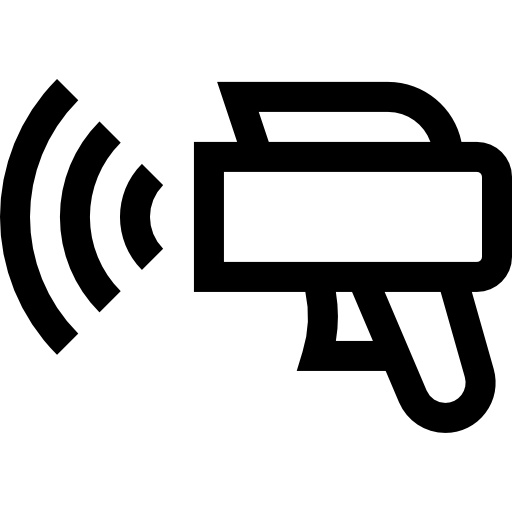
\includegraphics[width=1.5cm]{src/rapport_complet/img/radar-de-vitesse.png}}};
    % domain=1:7 -> dessine de x=1 à x=7
    % 0.2*sin(12*(\x-1.5) r) -> {Amplitude}*sin({Fréquence}*... r)
    \draw[black, thick, smooth] plot[domain=1:7, samples=1000] (\x, {0.4*sin(12*(\x-1.5) r)});
    \draw[-latex, thick] (7.5,0) -- ++(1,0) node[pos=0.5, above] {\(f_o\)};
    % --- Scénario 1 : Le véhicule s'approche ---
    \begin{scope}[yshift=1.5cm]
        % Onde réfléchie (fréquence plus élevée)
        \draw[black, thick, smooth] plot[domain=1:7, samples=1000] (\x, {0.4*sin(24*(\x-1) r)});
        \draw[-latex, thick] (0.5,0) -- ++(-1,0) node[pos=0.5, above] {\(f_o + f_d\)};
        \node (truck_approaching) at (9,0) {\scalebox{-1}[1]{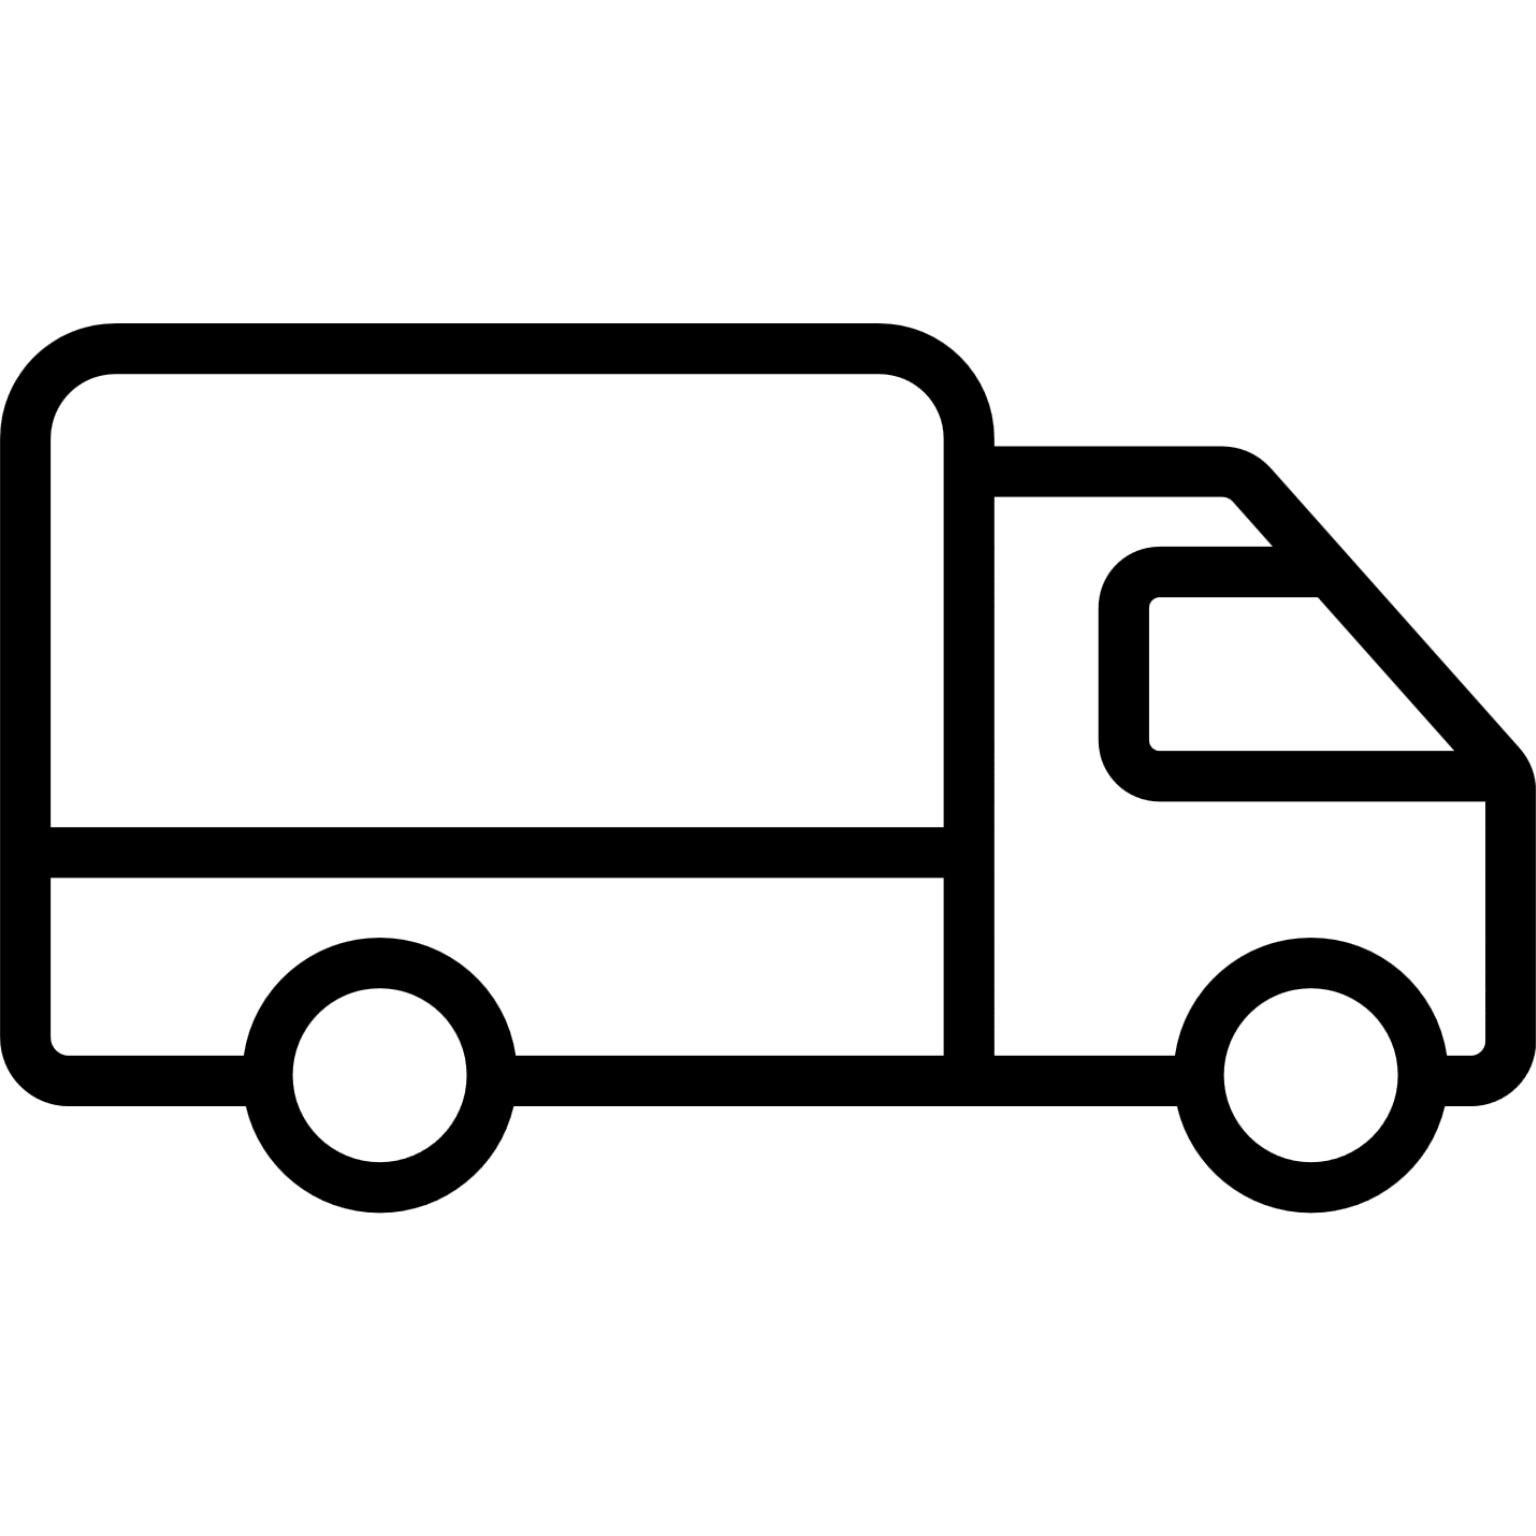
\includegraphics[width=1.5cm]{src/rapport_complet/img/truck-icon.png}}};
        \draw[-latex, thick] (truck_approaching) -- ++(-1.5,0);
    \end{scope}
    % --- Scénario 2 : Le véhicule s'éloigne ---
    \begin{scope}[yshift=-1.5cm]
        \node (truck_receding) at (8.25,0) {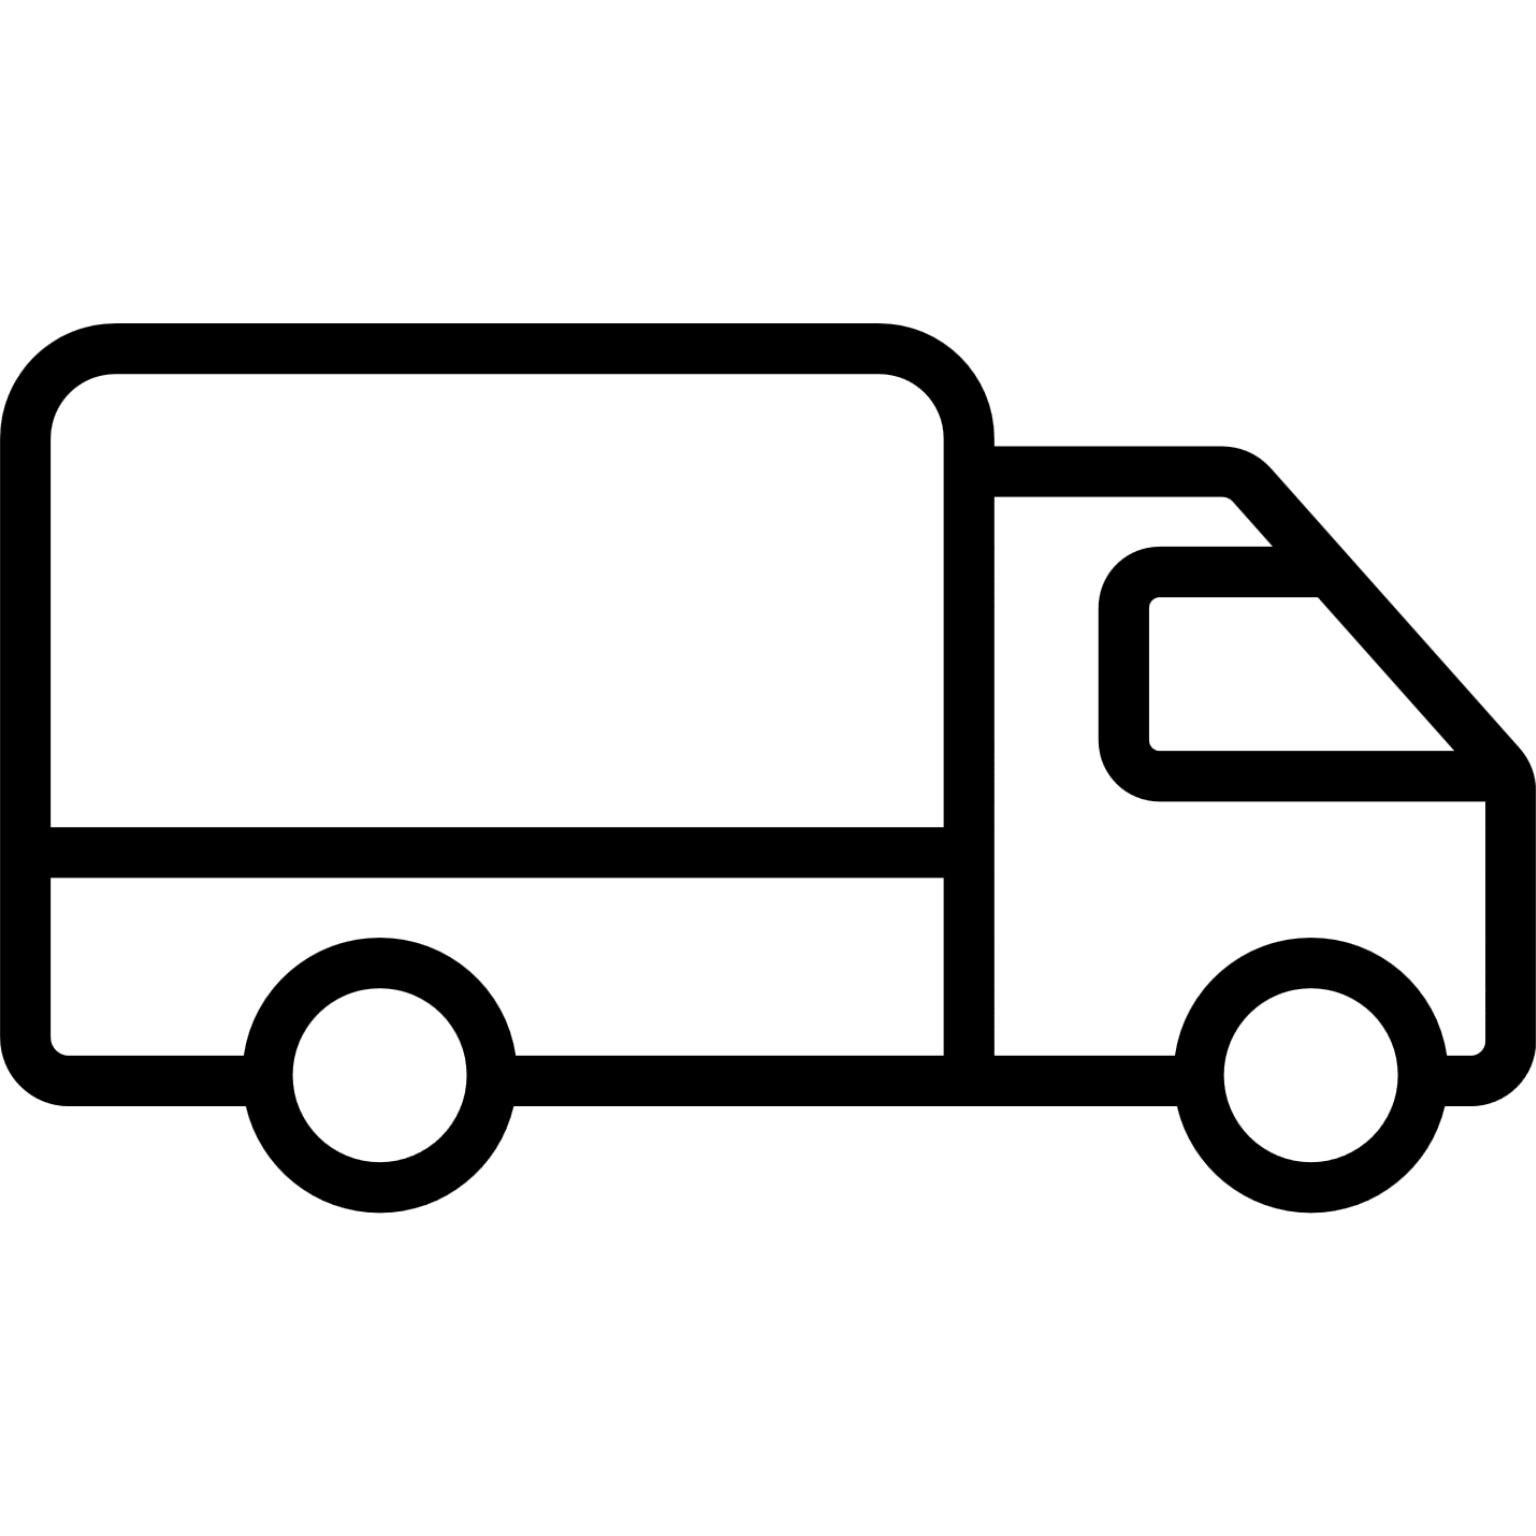
\includegraphics[width=1.5cm]{src/rapport_complet/img/truck-icon.png}};
        \draw[-latex, thick] (truck_receding) -- ++(1.5,0);
        % Onde réfléchie (fréquence plus basse)
        \draw[black, thick, smooth] plot[domain=1:7, samples=1000] (\x, {0.4*sin(6*(\x-1) r)});
        \draw[-latex, thin] (0.5,0) -- ++(-1,0) node[pos=0.5, below] {\(f_o - f_d\)};
    \end{scope}
    \end{tikzpicture}
    \caption{Illustration de l'effet Doppler-Fizeau}
    \label{fig:illustration_effet_doppler}
\end{figure}

\subsection{Formes d'ondes}\label{subsec:formes_ondes}

Au-delà de la géométrie et de la puissance, la nature du signal émis conditionne la portée, la résolution et la sensibilité. On distingue deux grandes catégories : impulsions simples et impulsions modulées.

\subsubsection{Impulsions simples}

Les impulsions courtes et puissantes (\emph{pulses}) sont suivies de périodes d’écoute pour capter les échos (voir figure \ref{fig:impulsions_radar_avec_echo}). La détection s’effectue via un filtre adapté, produisant un pic de corrélation dont le délai $\tau_e$ permet de calculer la distance, puisque la célérité du canal est connue \cite{richards2010}. La résolution en distance s’exprime :

\begin{equation}
    \delta_r \ge \frac{c_0 \cdot \tau_p}{2} = \frac{c_0}{2 \cdot B},
    \label{eq:resolution_distance_pulse}
\end{equation}
où $\tau_p$ est la durée de l’impulsion et $B$ sa bande de fréquence. Un compromis est nécessaire entre résolution en distance (favorisée par des impulsions courtes), résolution en vitesse (favorisée par des impulsions longues) et l'occupation spectrale (favorisée par des impulsions longues), cette dernière s’exprimant :

\begin{equation}
    \delta\nu_r = \frac{\lambda_0}{2\cdot\tau_p} = \frac{\lambda_0\cdot B}{2}.
    \label{eq:resolution_vitesse_impulsions}
\end{equation}
L’ambiguïté de portée maximale non ambiguë pour les radars à impulsion est donnée par \cite{skolnik2001,radartutorial} :

\begin{equation}
    R_{\max} = \frac{c_0\cdot(T_p - \tau_p)}{2}.
    \label{eq:resolution_distance_max_radar_pulse}
\end{equation}

\begin{figure}[htbp]
    \centering
    \begin{tikzpicture}[label/.style={font=\small}]
        % --- Définition des paramètres ---
        \def\periodeTp{7}             % Période de répétition des impulsions (Tp)
        \def\largeurImpulsion{0.3}    % Largeur de l'impulsion (τp)
        \def\retardEcho{4}            % Retard de l'écho (τe)
        \def\amplitudeEmise{3}        % Amplitude de l'impulsion émise
        \def\amplitudeEcho{0.5}       % Amplitude de l'écho
        \def\xstart{1}                % Position de départ pour le dessin
        % --- Dessin des axes ---
        \draw[-{Stealth[length=3mm]}, thick] (-0.5, 0) -- (\xstart+\periodeTp+\largeurImpulsion+1.5, 0) node[below] {$t$};
        \draw[-{Stealth[length=3mm]}, thick] (0, -1) -- (0, \amplitudeEmise+1) node[left] {Amplitude};
        \node[below left] at (0,0) {0};
        % --- Dessin des signaux ---
        % Ligne de base et impulsions émises (noir)
        \draw[thick] (\xstart-1, 0) -- (\xstart, 0)
            -- (\xstart, \amplitudeEmise) -- (\xstart+\largeurImpulsion, \amplitudeEmise) -- (\xstart+\largeurImpulsion, 0) -- (\xstart+\periodeTp, 0) -- (\xstart+\periodeTp, \amplitudeEmise) -- (\xstart+\periodeTp+\largeurImpulsion, \amplitudeEmise) -- (\xstart+\periodeTp+\largeurImpulsion, 0) -- (\xstart+\periodeTp+\largeurImpulsion+1, 0);
        % Impulsion de l'écho (rouge)
        \draw[thick, red] (\xstart+\retardEcho, 0) -- (\xstart+\retardEcho, \amplitudeEcho) -- (\xstart+\retardEcho+\largeurImpulsion, \amplitudeEcho) -- (\xstart+\retardEcho+\largeurImpulsion, 0);
        % --- Annotations ---
        % Annotation de Tp (Période de répétition)
        \draw[dashed, gray] (\xstart, \amplitudeEmise) -- (\xstart, \amplitudeEmise+0.5) -- (\xstart+\periodeTp, \amplitudeEmise+0.5) -- (\xstart+\periodeTp, \amplitudeEmise);
        \node[label, above] at (\xstart+\periodeTp/2, \amplitudeEmise+0.5) {$T_p$};
        % Annotation de τe (Retard de l'écho)
        \draw[dashed, gray] (\xstart+\largeurImpulsion, 0) -- (\xstart+\largeurImpulsion, -0.7) -- (\xstart+\retardEcho, -0.7) -- (\xstart+\retardEcho, 0);
        \node[label, below] at (\xstart+\largeurImpulsion+\retardEcho/2, -0.7) {$\tau_e$};
        % Annotation de τp (Largeur de l'impulsion) - CORRIGÉ
        \draw[dashed, gray] (\xstart, \amplitudeEmise) -- (\xstart, \amplitudeEmise+1) -- (\xstart+\largeurImpulsion, \amplitudeEmise+1) -- (\xstart+\largeurImpulsion, \amplitudeEmise);
        \node[label, above] at (\xstart+\largeurImpulsion/2, \amplitudeEmise+1) {$\tau_p$};
    \end{tikzpicture}
    \caption{Représentation d'impulsions simples avec un écho d'un radar}
    \label{fig:impulsions_radar_avec_echo}
\end{figure}

\subsubsection{Impulsions modulées}
La modulation linéaire (\emph{chirp} Sawtooth), illustrée en \ref{fig:impulsions_chirp_avec_echo} fait varier la fréquence sur une bande $B_{ch}$, améliorant le pic de corrélation pour la résolution en distance. C'est cette complexité spectrale (la large bande $B_ch$) qui permet, après corrélation, d'obtenir un pic fin proportionnel à $\frac{1}{B_ch}$, et non à la durée de l'impulsion :

\begin{equation}
    \delta_r = \frac{c_0}{2\cdot B_{ch}}.
    \label{eq:resolution_en_distance_chirp}
\end{equation}

Cependant, la superposition du décalage Doppler et de la dérive de fréquence induit une ambiguïté distance/vitesse \cite{cumming2005}.

\begin{figure}[htbp]
    \centering
    \begin{tikzpicture}[
        label/.style={font=\small, black},
        annotation/.style={black, thick},
        axis/.style={thick, gray!50!black}, % Couleur pour les axes
        gridline/.style={dashed, gray} % Style pour les lignes de grille/verticales
    ]
        % --- Définition des paramètres ---
        \def\Ts{3}       % Période de la rampe (T_s)
        \def\Bch{2.5}    % Bande passante / Amplitude (B_ch)
        \def\retard{0.6} % Retard temporel (\tau_e)
        \def\nramps{3}   % Nombre de rampes à dessiner
        % --- Dessin des axes ---
        % Axe horizontal (temps)
        \draw[-{Stealth[length=3mm]}, axis] (-0.5,0) -- (\nramps*\Ts + \Ts + 1,0) node[right,black] {$t$};
        % Axe vertical (fréquence)
        \draw[-{Stealth[length=3mm]}, axis] (0,-0.5) -- (0,\Bch + 0.8) node[above,black] {$f(t)$};
        \node[below left, black] at (0,0) {0};
        % --- Dessin des signaux et lignes verticales ---
        \foreach \i in {0,...,\nramps} {
            % Signal transmis (noir) - en dents de scie
            \draw[black, thick] (\i*\Ts, 0) -- (\i*\Ts + \Ts, \Bch);
            % Lignes verticales pour le signal noir
            \ifnum\i<\nramps % Ne pas dessiner la dernière ligne verticale si elle sort du graphique
                \draw[black, thick] (\i*\Ts + \Ts, 0) -- (\i*\Ts + \Ts, \Bch);
            \fi
        }
        \foreach \i in {0,...,\nramps} {
            % Signal écho (rouge) - retardé dans le temps
            \draw[red, thick] (\i*\Ts + \retard, 0) -- (\i*\Ts + \Ts + \retard, \Bch);
             % Lignes verticales pour le signal rouge
             % On peut ajouter une condition si on ne veut pas qu'elles s'étendent trop loin
             \ifnum\i<\nramps % Ne pas dessiner la dernière ligne verticale si elle sort du graphique
                 \draw[red, thick] (\i*\Ts + \Ts + \retard, 0) -- (\i*\Ts + \Ts + \retard, \Bch);
             \fi
        }
        % --- Annotations ---
        % Annotation \tau_e (Retard temporel)
        \draw[<->, annotation] (0, -0.3) -- (\retard, -0.3) node[midway, below, label] {$\tau_e$};
        % Annotation T_s (Période)
        % On la place au-dessus, entre le début de la 2ème et 3ème rampe
        \draw[<->, annotation] (\Ts, \Bch+0.3) -- (2*\Ts, \Bch+0.3) node[midway, above, label] {$T_s$};
        % Annotation B_ch (Bande passante)
        % On la place à droite pour correspondre à l'image
        \draw[<->, annotation] (-0.25, 0) -- (-0.25, \Bch) node[midway, left, label] {$B_{ch}$};
        % Annotation \Delta f = f_b (Fréquence de battement)
        % On choisit un point dans le temps pour montrer la différence de fréquence
        % Positionnée au milieu de la 3ème rampe noire
        \def\annotXpos{2*\Ts + 0.5*\Ts} 
        % Coordonnée sur le signal noir à x = \annotXpos
        % La rampe n°2 (i=2) va de x=2*Ts à 3*Ts. L'équation est y = (Bch/Ts) * (x - 2*Ts)
        \coordinate (point_noir) at (\annotXpos, {(\Bch/\Ts) * (\annotXpos - 2*\Ts)});
        % Coordonnée sur le signal rouge à x = \annotXpos
        % L'écho de la rampe n°2 va de x=2*Ts+retard à 3*Ts+retard. L'équation est y = (Bch/\Ts) * (x - retard - 2*\Ts)
        \coordinate (point_rouge) at (\annotXpos, {(\Bch/\Ts) * (\annotXpos - \retard - 2*\Ts)});
        \draw[<->, annotation] (point_rouge) -- (point_noir) node[midway, below right, label] {$\Delta f = f_b$};
    \end{tikzpicture}
    \caption{Représentation d'une impulsion Chirp et d'un écho}
    \label{fig:impulsions_chirp_avec_echo}
\end{figure}

La modulation triangulaire FMCW, illustrée figure \ref{fig:fmcw_avec_echo}, émet alternativement des chirps ascendants et descendants. En mesurant deux fréquences de battement distinctes, on dissocie sans ambiguïté portée et vitesse \cite{richards2010}.

\FloatBarrier
\begin{figure}[htbp]
    \centering
    \begin{tikzpicture}[label/.style={font=\small}]
        % --- Définition des paramètres ---
        \def\Tr{5}      % Période de la rampe (T_r)
        \def\Amp{2.5}    % Amplitude (correspond à B_ch / 2)
        \def\retard{0.8} % Retard temporel (\tau_e)
        \def\doppler{0.3} % Décalage en fréquence (f_d)
        % --- Dessin des axes ---
        \draw[-{Stealth[length=3mm]}, thick] (-0.5,0) -- (2.2*\Tr,0) node[right] {$t$};
        \draw[-{Stealth[length=3mm]}, thick] (0,-0.5) -- (0,\Amp+1) node[above] {$f(t)$};
        \node[below left] at (0,0) {0};
        % --- Signal transmis (en bleu) ---
        \draw[black, thick] (0,0) -- (\Tr/2, \Amp) -- (\Tr, 0) -- (1.5*\Tr, \Amp) -- (2*\Tr, 0);
        % --- Signal reçu (en rouge) ---
        \draw[red, thick] (\retard, \doppler) -- (\Tr/2+\retard, \Amp+\doppler) -- (\Tr+\retard, \doppler) -- (1.5*\Tr+\retard, \Amp+\doppler) -- (2*\Tr+\retard, \doppler);
        % --- Annotations et lignes de repère ---
        % Lignes pointillées et ticks sur l'axe des temps (VERSION SIMPLIFIÉE)
        \foreach \pos/\labeltext in {\retard/\tau_e, \Tr/T_r} {\draw[dashed, gray] (\pos, -0.1) -- (\pos,0);\node[below, label] at (\pos, -0.1) {$\labeltext$};}
        % Annotation de B_ch
        \draw[<->, thick] (-0.3, 0) -- (-0.3, \Amp) node[midway, left, label] {$B_{ch}$};
        % --- Annotation du retard (\tau) ---
        % Lignes pointillées partant du sommet de chaque signal
        \draw[dashed, gray] (\Tr/2, \Amp) -- (\Tr/2, \Amp+1); % Ligne du pic bleu
        \draw[dashed, gray] (\Tr/2+\retard, \Amp+\doppler) -- (\Tr/2+\retard, \Amp+1); % Ligne du pic rouge
        % Ligne horizontale supérieure et le label
        \draw[dashed, gray] (\Tr/2, \Amp+1) -- (\Tr/2+\retard, \Amp+1);
        \node[above, label] at (\Tr/2+\retard/2, \Amp+1) {$\tau_e$};
        % --- Annotation de f_d ---
        \def\fdXpos{\Tr/2+\retard+1} % Position en x de la flèche f_d (décalée de 1)
        % Ligne pointillée du pic bleu jusqu'à la flèche f_d
        \draw[dashed, gray] (\Tr/2, \Amp) -- (\fdXpos, \Amp);
        % Ligne pointillée du pic rouge jusqu'à la flèche f_d
        \draw[dashed, gray] (\Tr/2+\retard, \Amp+\doppler) -- (\fdXpos, \Amp+\doppler);
        % La flèche f_d, décalée vers la droite
        \draw[<->] (\fdXpos, \Amp) -- (\fdXpos, \Amp+\doppler) node[midway, right, label] {$f_d$};
        % Annotation des fréquences de battement (fb_up et fb_dw)
        % f_b^up
        \def\upPos{1.5} % Position en x pour l'annotation
        \coordinate (A) at (\upPos, {(\Amp/(\Tr/2))*(\upPos - \retard) + \doppler});
        \coordinate (B) at (\upPos, {(\Amp/(\Tr/2))*\upPos});
        \draw[<->, thick] (A) -- (B) node[midway, below right, label] {$f_b^{up}$};
        % f_b^dw
        \def\dwPos{4} % Position en x pour l'annotation
        \coordinate (C) at (\dwPos, {\Amp+\doppler - (\Amp/(\Tr/2))*(\dwPos - \Tr/2 - \retard)});
        \coordinate (D) at (\dwPos, {\Amp - (\Amp/(\Tr/2))*(\dwPos - \Tr/2)});
        \draw[<->, thick] (C) -- (D) node[midway, below right, label] {$f_b^{dw}$};
    \end{tikzpicture}
    \caption{Représentation de la forme d'onde FMCW et d'un écho}
    \label{fig:fmcw_avec_echo}
\end{figure}
\FloatBarrier

\noindent Les résolutions s’expriment alors \cite{richards2010} :

\begin{equation}
    \delta_r = \frac{c_0}{2\cdot B_{ch}},
    \label{eq:resolution_distance_fmcw_triangulaire}
\end{equation}

\begin{equation}
    \delta\nu_r = \frac{c_0}{2\cdot f_0\cdot T_r}.
    \label{eq:resolution_vitesse_fmcw_triangulaire}
\end{equation}

Cet équilibre favorable est contrebalancé par la complexité matérielle accrue, surtout sur de larges bandes \cite{meta2007performance}.

On remarque ainsi que les deux résolutions ne sont pas inversement liées. On peut donc avoir une bonne résolution en distance et une bonne résolution en vitesse. Cependant, cet avantage doit être nuancé par la complexité de la réalisation matérielle de cette forme d'onde, d'autant plus sur une large bande \cite{meta2007performance}. 

\subsection{Bases du bruit}

Jusqu’à présent, le bruit a été négligé. Or, il est indispensable de le caractériser pour évaluer la performance réelle. Le signal désigne les échos utiles, tandis que le bruit englobe toutes les perturbations (interférences, hydrométéores, bruit thermique des composants). Le rapport signal-sur-bruit (SNR) se définit \cite{skolnik2001} :

\begin{equation}
    SNR = \frac{P_{signal}}{P_{bruit}},
    \label{eq:snr}
\end{equation}
et le facteur de bruit d’un dispositif, selon Friis \cite{skolnik2001,Friis1944Noise}, :

\begin{equation}
    F = \frac{(S/N)_e}{(S/N)_s} = \frac{N_s}{G\cdot N_e}.
    \label{eq:facteur_de_bruit}
\end{equation}
Où :
\begin{description}
    \item[$F$] : Le facteur de bruit
    \item[$S$] : La puissance du signal [$W$]
    \item[$N_x$] : La puissance du bruit, en entrée pour $x=e$, en sortie pour $x=s$ [$W$]
    \item[$G$] : Le gain du dispositif traversé
\end{description}
\vspace{1em}

Le facteur de bruit représente donc le rapport entre le RSB en entrée et le RSB en sortie. La deuxième partie de l'équation permet de définir $F$ par rapport à une référence de bruit thermique en entrée à $T_0 = 290 \degree K$, tel que $N_e = k\cdot T_0 \cdot B$ avec $k$ la constante de Boltzmann et $B$ la bande de fréquence observée. On définit alors la température équivalente de bruit \cite{Friis1944Noise} :

\begin{equation}
    T_{eq} = (F-1)\cdot T_0 .
    \label{eq:temp_eq_de_bruit}
\end{equation}
Où :
\begin{description}
    \item[$T_{eq}$] : La température équivalente de bruit [$\degree K$] 
    \item[$F$] : Le facteur de bruit
    \item[$T_0$] : La température de référence ($290 \degree K$) [$\degree K$]
\end{description}
\vspace{1em}

La figure \ref{fig:snr_degradation} illustre l'évolution du SNR à travers de la chaîne RF présentée par la figure \ref{fig:illus_snr_facteur_de_bruit}. Elles montrent l'importance du premier élément dans la performance globale du système.

\FloatBarrier
\begin{figure}[htbp]
    \centering
    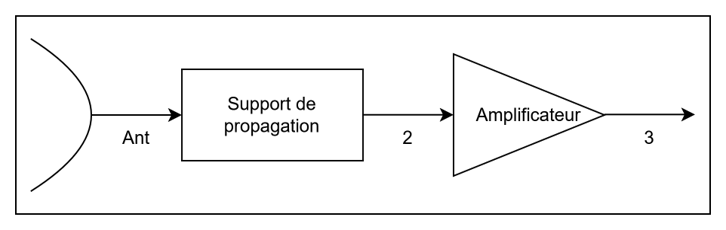
\includegraphics[width=0.5\linewidth]{src/rapport_complet/img/schema_facteur_bruit.png}
    \caption{Système permettant l'explication du SNR et du facteur de bruit}
    \label{fig:illus_snr_facteur_de_bruit}
\end{figure}
\FloatBarrier

\begin{figure}[htbp]
    \centering 
    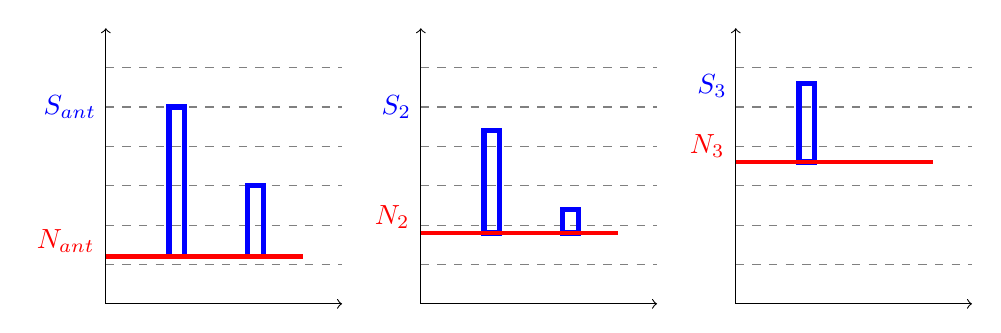
\begin{tikzpicture}
        % Graphique 1 : Bon rapport S/B
        \begin{scope}[xshift=0cm]
            % Axes
            \draw[->] (0,0) -- (3,0);
            \draw[->] (0,0) -- (0,3.5);
            % Lignes de référence signal
            \foreach \y in {0.5, 1.0, 1.5, 2.0, 2.5, 3.0} {
                \draw[dashed, gray] (0,\y) -- (3,\y);
            }
            % Signal (S_ant)
            \draw[line width=2pt, blue] (0.8,0.6) rectangle (1.0,2.5);
            \draw[line width=2pt, blue] (1.8,0.6) rectangle (2.0,1.5);
            \node[left, blue, yshift=-0.5cm] at (0,3) {$S_{ant}$};
            % Bruit (N_ant)
            \draw[line width=1.5pt, red] (0,0.6) -- (2.5,0.6) node[left, red, xshift=-2.5cm, yshift=0.2cm] {$N_{ant}$};
        \end{scope}
        % Graphique 2 : Rapport S/B dégradé
        \begin{scope}[xshift=4cm]
            % Axes
            \draw[->] (0,0) -- (3,0);
            \draw[->] (0,0) -- (0,3.5);
            % Lignes de référence signal
            \foreach \y in {0.5, 1.0, 1.5, 2.0, 2.5, 3.0} {
                \draw[dashed, gray] (0,\y) -- (3,\y);
            }
            % Signal (S2)
            \draw[line width=2pt, blue] (0.8,0.9) rectangle (1.0,2.2);
            \draw[line width=2pt, blue] (1.8,0.9) rectangle (2.0,1.2);
            \node[left, blue, yshift=-0.5cm] at (0,3) {$S_2$};
            % Bruit (N2)
            \draw[line width=1.5pt, red] (0,0.9) -- (2.5,0.9) node[left, red, xshift=-2.5cm, yshift=0.2cm] {$N_2$};
        \end{scope}
        % Graphique 3 : Rapport S/B fortement dégradé
        \begin{scope}[xshift=8cm]
            % Axes
            \draw[->] (0,0) -- (3,0);
            \draw[->] (0,0) -- (0,3.5);
            % Lignes de référence signal
            \foreach \y in {0.5, 1.0, 1.5, 2.0, 2.5, 3.0} {
                \draw[dashed, gray] (0,\y) -- (3,\y);
            }
            % Signal (S3)
            \draw[line width=2pt, blue] (0.8,1.8) rectangle (1,2.8);
            % Le deuxième pic est trop proche du bruit pour être clairement visible
            \node[above, blue, xshift=-0.3cm, yshift=-0.5cm] at (0,3) {$S_3$};
            % Bruit (N3)
            \draw[line width=1.5pt, red] (0,1.8) -- (2.5,1.8) node[left, red, xshift=-2.5cm, yshift=0.2cm] {$N_3$};
        \end{scope}
    \end{tikzpicture}
    \caption{Illustration de la dégradation du SNR au travers d'un système}
    \label{fig:snr_degradation}
\end{figure}

\noindent Le gain total d’une chaîne de $n$ éléments s’exprime par \cite{Friis1944Noise} :
\begin{equation}
    G_T = \prod_{i=1}^n G_i,
    \label{eq:gain_total}
\end{equation}
et le facteur de bruit total par la formule de Friis :
\begin{equation}
    F_T = F_1 + \sum_{i=2}^n \frac{F_i - 1}{\prod_{k=1}^{i-1} G_k}.
    \label{eq:formule_friis_bruit}
\end{equation}

La sélection soignée du premier composant est cruciale pour limiter la dégradation globale du SNR. Avec ces notions établies, la section \ref{sec:principes_sar} détaillera les principes spécifiques à l’imagerie radar, en particulier le SAR.

% \subsection{Architecture matérielle}
% % Pertinence ? Si oui à quel niveau on descend ?

\subsection{Applications}

Les radars pulsés occupent une place centrale dans la surveillance à grande échelle. Grâce à leur capacité à mesurer avec précision la distance et la vitesse des cibles, ils sont largement utilisés dans la surveillance aérienne, les relevés météorologiques et les systèmes de navigation. Leur principe, basé sur l’émission brève d’impulsions suivie d’une mesure du temps d’écho, constitue également la base de nombreuses techniques d’imagerie haute résolution, comme le radar à synthèse d’ouverture (SAR). 

Les radars à onde Sawtooth sont privilégiés dans des contextes nécessitant une observation continue et fiable, tels que la surveillance maritime ou certaines applications industrielles. Leur modulation linéaire en fréquence permet une estimation stable des distances et des vitesses, essentielle à la détection d’objets mobiles dans des environnements complexes.

Enfin, les systèmes FMCW triangulaires se distinguent par leur précision et leur compacité. Utilisés dans les radars de contrôle de la circulation, les systèmes anticollision et les capteurs de distance, ils offrent des mesures fines de portée tout en s’adaptant aux environnements dynamiques. 

L’exploitation de ces différentes formes d’ondes trouve un prolongement naturel dans les applications d’imagerie radar, où la combinaison de résolutions spatiale et temporelle permet de reconstituer des représentations détaillées des scènes observées.

